\Subhead{1.2.1}{Автоколебательная система с одной степенью свободы}
\textbf{Определение.} Автоколебания --- поддерживаемые системой колебания, получающие энергию от непериодического источника; момент её подачи определяется обратной связью самого движения. При вынужденных колебаниях ритм задаёт внешняя периодическая сила; здесь он возникает внутри системы.

В LC-генераторе колебательный контур задаёт частоту, источник питания даёт энергию, транзистор с обратной связью подаёт её в нужной фазе. В часах аналогичную роль играет анкер. Для конечной устойчивой амплитуды необходима нелинейность: линейное отрицательное трение даёт неограниченный рост, а точно нулевое затухание --- семейство амплитуд, зависящих от начального состояния.

Размерная модель Ван-дер-Поля:
\begin{equation}\label{eq:vdp}
 \ddot x-2\mu(1-x^2/a^2)\dot x+\omega_0^2x=0,
 \qquad \mu>0.
\end{equation}
$a$ задаёт масштаб координаты, $\mu$ имеет размерность с$^{-1}$. При малом $|x|$ энергия подкачивается, при большом отбирается. В слабонелинейном случае $\mu\ll\omega_0$ режим почти синусоидален. Сильная нелинейность может давать релаксационные колебания: медленное накопление и быстрый сброс энергии.

На фазовой плоскости устойчивым периодическим автоколебаниям соответствует \emph{предельный цикл}, изолированная замкнутая орбита. Соседние траектории притягиваются к ней; фаза вдоль орбиты остаётся свободной. Амплитуда и частота не зависят от начальных условий \emph{внутри области притяжения данного режима}. При нескольких аттракторах итог зависит от начального состояния.
\begin{center}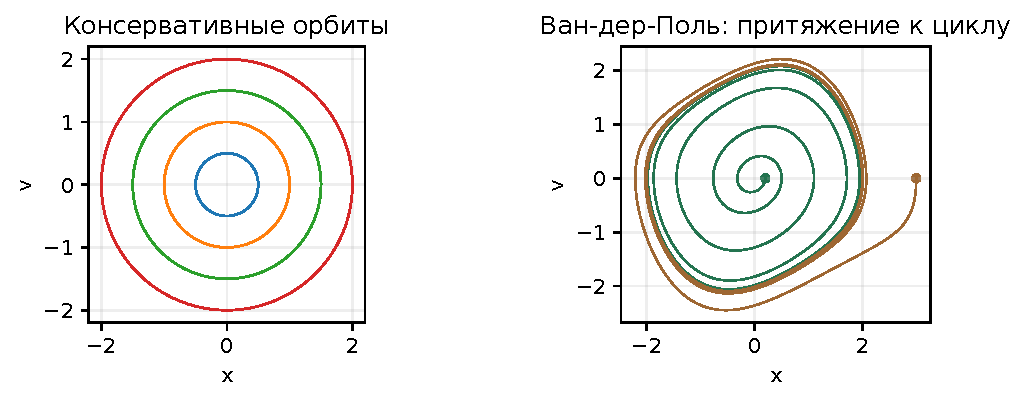
\includegraphics[width=.72\linewidth]{figures/limit_cycle.pdf}\end{center}
